
\documentclass{article}

\usepackage{physics}

\setlength{\oddsidemargin}{0 in}
\setlength{\topmargin}{-0.6 in}
\setlength{\textwidth}{6.5 in}
\setlength{\textheight}{8.5 in}
\setlength{\headsep}{0.75 in}
\setlength{\parindent}{0 in}
\setlength{\parskip}{0.1 in}

%
% ADD PACKAGES here:
%

\usepackage{amsmath,amsfonts,graphicx}

\newcounter{lecnum}

%
% The following macro is used to generate the header.
%
\newcommand{\lecture}[4]{
   \pagestyle{myheadings}
   \thispagestyle{plain}
   \newpage
   \setcounter{lecnum}{#1}
   \setcounter{page}{1}
   \noindent
   \begin{center}
   \framebox{
      \vbox{\vspace{2mm}
    \hbox to 6.28in { {\bf CC484: Pattern Recognition
	\hfill Spring 2018} }
       \vspace{4mm}
       \hbox to 6.28in { {\Large \hfill Sheet #1: #2  \hfill} }
       \vspace{2mm}
       \hbox to 6.28in { {\it #3 \hfill #4} }
      \vspace{2mm}}
   }
   \end{center}
   \markboth{Sheet #1: #2}{Sheet #1: #2}
}

\newcommand\E{\mathbb{E}}


%%%%%%%%%%%%%%%%%%%%%%%%%%%%%%%%%%%%%%%%%%%%%%%%%%%%%%%%%%%%%%%%%%%%%%%%%%%%%%%%%%%%%%



\begin{document}
%FILL IN THE RIGHT INFO.
%\lecture{**Sheet-NUMBER**}{**Title**}{**Name**}{**Date**}
\lecture{3}{Normailzed Cuts and Similarity Graphs}{Abdelrahman Mohamed Abdelnabi, 3466}{May 17}

\section{Normalized Cut}

The cost of a graph partition into two sets A and B is the sum of the weights of edges connecting vertices in A with vertices in B.

$$cut(A,B) = \sum_{i \in A, j \in B} W_{ij}$$

This cost function however, will often isolate vetrices because vertice with a small degree when cut, will have a low cost. To avoid this problem, we use the normalized cut cost funtion, which aims to partition the graph into two nearly equal partitions in size.

$$NCut(A, B) = cut(A,B)(\frac{1}{vol(A)} + \frac{1}{vol(B)})$$
\begin{center}
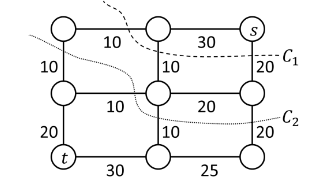
\includegraphics[width=0.5\linewidth]{graph.png}
\end{center}

\begin{enumerate}
\item Using the un-normalized min cut. The cost of cut $C_1$ is

$$C_1 = 10 + 10 + 20 = 40$$

and the cost of $C_2$ is

$$C_2 = 10 + 10 + 10 + 20 = 50$$

The un-normalized min cut cost function gives a lower cost to $C_1$ than to to $C_2$.

\item When using the normalized cut. $vol(C_i)$ is defined as the sum of all the weights on edges with one end in cluster $C_i$

$$vol(C_i) = \sum_{v_j \in C_i} d_j$$

For cut $C_1$, $vol(A) = 100$ and $vol(B) = 280$ and for cluster $C_2$, $vol(A) = 230$ and $vol(B) = 200$. The cost of $C_1$ is

$$C_1 = 40(\frac{1}{100} + \frac{1}{280}) = 0.542$$

and the cost of $C_2$ is

$$C_2 = 50(\frac{1}{230} + \frac{1}{200}) = 0.467$$

The normalized cut cost of cut $C_2$ is lower than that of $C_1$ which is what we want for clustering.

\end{enumerate}


\end{document}